% \iffalse meta-comment
%
% Copyright 1993 1994 1995 1996 1997 1998 1999 2000 2001
% The LaTeX3 Project and any individual authors listed elsewhere
% in this file. 
% 
% This file is part of the LaTeX base system.
% -------------------------------------------
% 
% It may be distributed and/or modified under the
% conditions of the LaTeX Project Public License, either version 1.2
% of this license or (at your option) any later version.
% The latest version of this license is in
%    http://www.latex-project.org/lppl.txt
% and version 1.2 or later is part of all distributions of LaTeX 
% version 1999/12/01 or later.
% 
% The list of all files belonging to the LaTeX base distribution is
% given in the file `manifest.txt'. See also `legal.txt' for additional
% information.
% 
% \fi
% Filename: usrguide.tex

%\NeedsTeXFormat{LaTeX2e}[1995/12/01]
\documentclass[a4paper,twoside]{article}
\usepackage{geometry}
\geometry{left=2.5cm,right=2.5cm,top=2.5cm,bottom=2.5cm}
\usepackage[UTF8]{ctex}
\usepackage[siunitx]{circuitikz}
\usepackage{tikz}
\usepackage{blindtext}
\usepackage[colorlinks,urlcolor=blue]{hyperref}
\usepackage{listings}
\usepackage{color}
\lstset{breaklines}%这条命令可以让LaTeX自动将长的代码行换行排版
\lstset{extendedchars=false}%这一条命令可以解决代码跨页时,章节标题,页眉等汉字不显示的问题
\graphicspath{{figures/}}
\title{Cadence Allegro技巧}

\author{\href{mailto:wyu0831@hotmail.com}{Wang Yu}\\ Department of Modern Physics, USTC}

\date{\today}


\begin{document}

\maketitle

% \tableofcontents

\abstract{说明}
本文档用于记录平时使用Allegro的技巧,做为胡佳栋教程的补充
\clearpage
\tableofcontents
\clearpage
\section{制作LOGO}
	\begin{enumerate}
		\item 需要准备一张bmp格式的图片,如下图所示 \\ 
\includegraphics[width=0.3\textwidth]{figures/SDHCALFEB1V0.png}
		\item 新建一个Format Symbol \\ 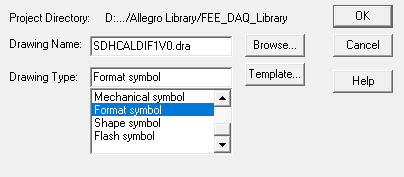
\includegraphics[width=0.6\textwidth]{figures/CreateFormatSymbol.png}
		\item 设置好画布和栅格点大小,按照经验最后LOGO的大小是画布大小的一半,按照自己需要的大小设置栅格点即可
		\item 选择File $\rightarrow$ Import $\rightarrow$ Logo,并按照下图所示设置 \\ 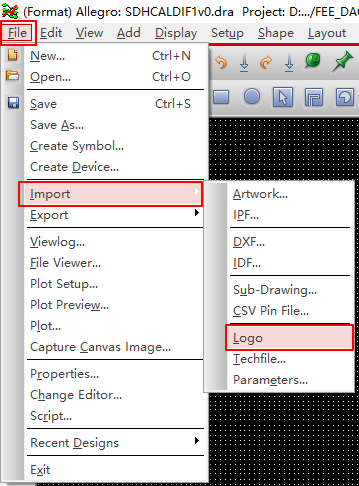
\includegraphics[width= 0.3\textwidth]{figures/FileImportLogo.png} 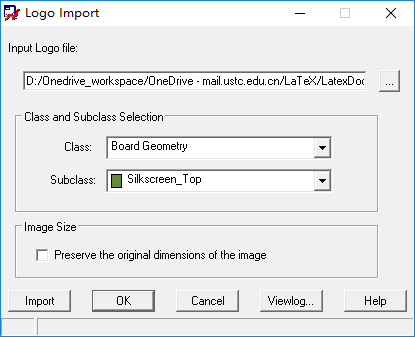
\includegraphics[width=0.3\textwidth]{figures/LogoImport.png}
		\item 使用命令 Shape $\rightarrow$ Compose Shape 并在Option中设置Class和Subclass分别为Board Geometry和Silkscreen\_Top \\ 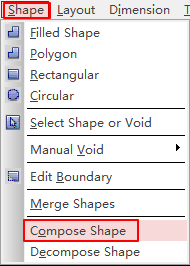
\includegraphics[width=0.4\textwidth]{figures/ShapeComposeShape.png} 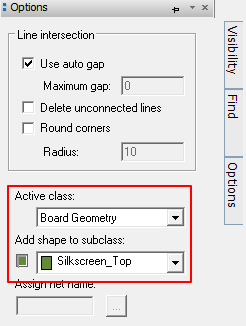
\includegraphics[width=0.4\textwidth]{figures/OptionClassAndSubClass.png}
		\item 保存。大功告成了
	\end{enumerate}

\section{Skill教程}
	\subsection{Allegro skill介绍}
		\begin{itemize}
			\item Skill 是Cadence 提供的可第二次开发的语言。语法同C语言类似。在设计中使用skill可以大大简化PCB绘制流程,还可以定制各种各样的功能
			\item 本文只对skill使用做一个简单的介绍,进阶的方面以后学会再做笔记
			\item 推荐一个网站:\href{http://www.allegro-skill.com/?fromuid=7754}{Allegro Skill},使用的skill和介绍均来自此网站
		\end{itemize}

	\subsection{Allegro skill设置方法}
	以一个skill为例(ch\_via\_net),这个skill的功能是将电路板中的过孔的网络修改为任意一个网络。
		\begin{enumerate}
			\item 先从任何一个地方获取到这个skill文件ch\_via\_net.il
			\item 将文件放置在一个文件夹中,不含中文和空格。如我放置在D:\textbackslash Cadence\textbackslash{skill}中,方便日后管理
			\item 在环境变量文件夹中找到allegro.ilinit文件,这个文件一般在C:\textbackslash Users\textbackslash\*\textbackslash AppData\textbackslash Roaming\textbackslash SPB\_Data\textbackslash pcbenv中,\*表示计算机用户名。
			\item 编辑这个文件,在文件中加入如下的代码
			\begin{lstlisting}
setSkillPath(buildString(append1(getSkillPath() "D:/Cadence/skill"))) ;设置skill所在路径
load("ch_via_net.il" "www.allegro-skill.com")
			\end{lstlisting};载入skill 前一个参数是skill文件,后一个是密码。
			\item Skill设计结束,可以在工程中使用了。
			\item 最好为skill的操作设置一个快捷键,不然使用中不会很方便。
			\item 可以自定义allegro菜单,将自己添加的skill加入菜单中方便使用
  				在安装路径D:\textbackslash Cadence\textbackslash SPB\_16.6\textbackslash share\\textbackslash pcb\textbackslash text\textbackslash cuimenus中找到allegro.men文件,该文件为加载目录文件。在目录的最后一个end前加入如下代码:
  		\begin{lstlisting}
POPUP "My_Skill"
	BEGIN
	MENUITEM "&Chang Via's Net",  "ch_via_net"
	END
		\end{lstlisting}
		\end{enumerate}



	\subsection{AlignTool}
	安装方法:
	\begin{enumerate}
		\item 下载AlignTool1.0.zip并解压到电脑中。
		\item 在解压出来的文件夹中直接点击install.bat进行安装,不需要手动进行安装。
		\item 重启allegro,输入命令aln运行。 
	\end{enumerate}


\section{制作异形过孔}
看图不说话\\ 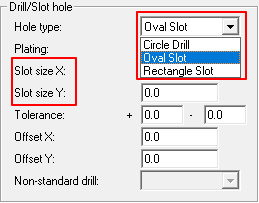
\includegraphics[width=0.3\textwidth]{figures/EvenViaSetting.png}

\section{从之前的工程中导入光绘设置}
在画电路板完成后需要生成光绘文件,如果每次都手动添加光绘设置会显得非常细碎,同时可能会有失误,如果此时正好有一个相同层数且布局相同的.brd文件,就可以从中导出以前的光绘设置,大大减少工作量。
下面就是操作步骤
\begin{enumerate}
	\item 先打开已经生成过光绘的.brd工程的生成光绘页面
	\item 点击Select all选中所有的光绘层,然后对着其中一个层右键单击
	\item 在出现对话框中选择Save All Checked
	\item Allegro会在工程文件夹下面生成一个FILM\_SETUP.txt的文件,这便是我们需要的文件,复制到新的工程目录下
	\\ 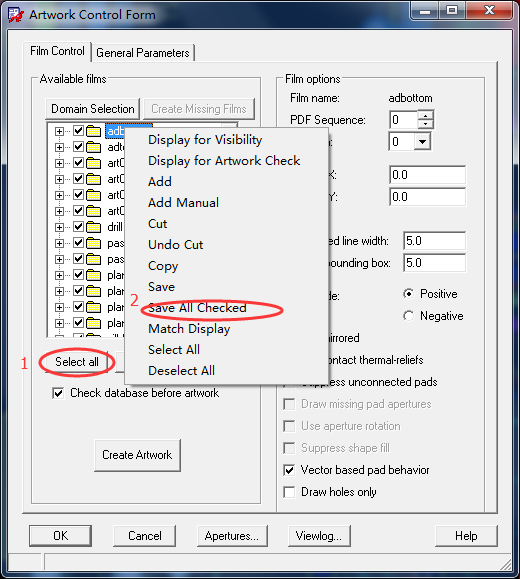
\includegraphics[width=0.3\textwidth]{figures/ArtworkSaveAllCheck.png}
	\item 在新的工程中生成光绘页面点击Add,在弹出对话框中选择刚刚复制过来的FILM\_SETUP.txt,光绘设置即被成功导入
	\\ 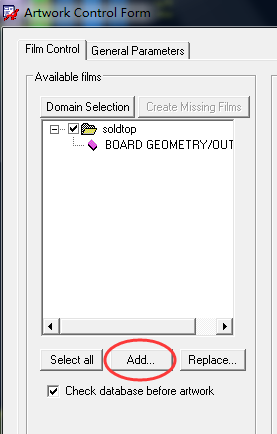
\includegraphics[width=0.3\textwidth]{figures/ArtworkAdd.png} 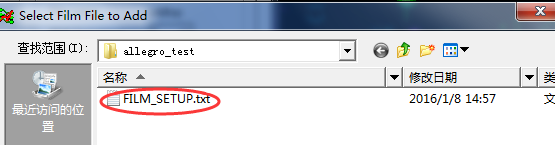
\includegraphics[width=0.3\textwidth]{figures/ArtworkSelectSetting.png}

\end{enumerate}
\section{新建SubClass}
Allegro自己默认了许多的Class和Subclass,这些Subclass都是在画电路板的时候必须的。有的时候画电路板需要一些辅助线,比如说分割FPGA的bank,摆放器件的时候也需要一些辅助线。以前的做法是放在丝印层,但是这种方法并不是设计安全的,如果忘记删除,会留下一些不好看的痕迹,最好的做法是创建一个自己的Subclass来摆放它们,下面是如何自定义Subclass
\begin{enumerate}
	\item 在Setup$\rightarrow$Subclasses中 \\ 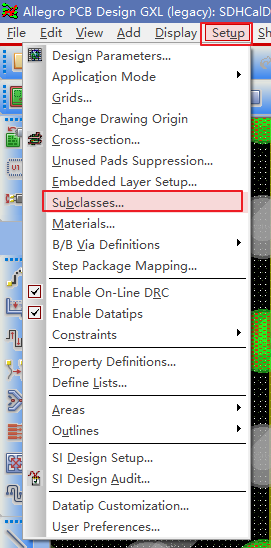
\includegraphics[width=0.3\textwidth]{figures/SetupSubclass.png}
	\item 然后在弹出的窗口中选择一个Class点击,然后在弹出的框中的New Subclass中填入自定义的Subclass的名称 \\ 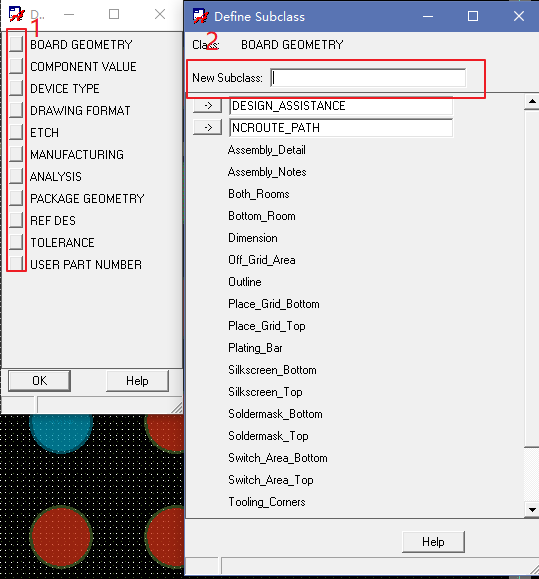
\includegraphics[width=0.3\textwidth]{figures/NewSubclass.png}
\end{enumerate}

\section{Allegro设置快捷键}
Allegro中本身默认了一些快捷键,但是使用起来不太方便,大多需要两个键一起组合,本教程介绍如何修改快捷键
	\subsection{快捷键介绍}
	先说一下Allegro的变量文件,一共有2个,一个是用户变量,一个是全局变量。
	用户变量文件的位置,通过系统环境变量设置:系统属性-高级-环境变量,其中的Home值就是env所在目录。要注意的是,这里也有两个变量,一个是用户变量一个是系统变量,在用户变量里设置了Home之后就不需要在系统变量里再设置了,如果同时设置的话,会以用户变量的为准而忽略系统变量。
	\\ 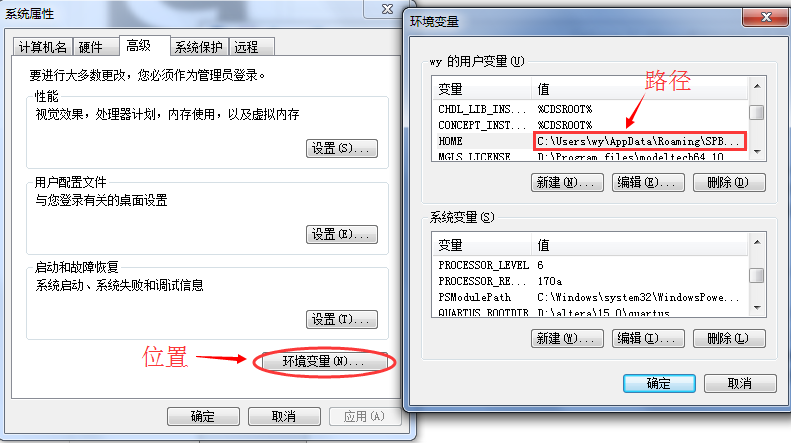
\includegraphics[width=0.4\textwidth]{figures/SystemEnviroment.png}
	\subsection{修改快捷键}
	\begin{enumerate}
		\item 在C:\textbackslash Users\textbackslash $\star$ \textbackslash AppData\textbackslash Roaming\textbackslash SPB\_Data\textbackslash pcbenv下面,编辑env文件,用任意文档编辑器打开即可,$\star$是用户名
		\item 修改快捷键有两个命令一个是alias,另一个是funckey,
		\item alias可以用来指定除字母以外的其他按键,举例如下
	\end{enumerate}
	下面是我的一些快捷键
	\\ 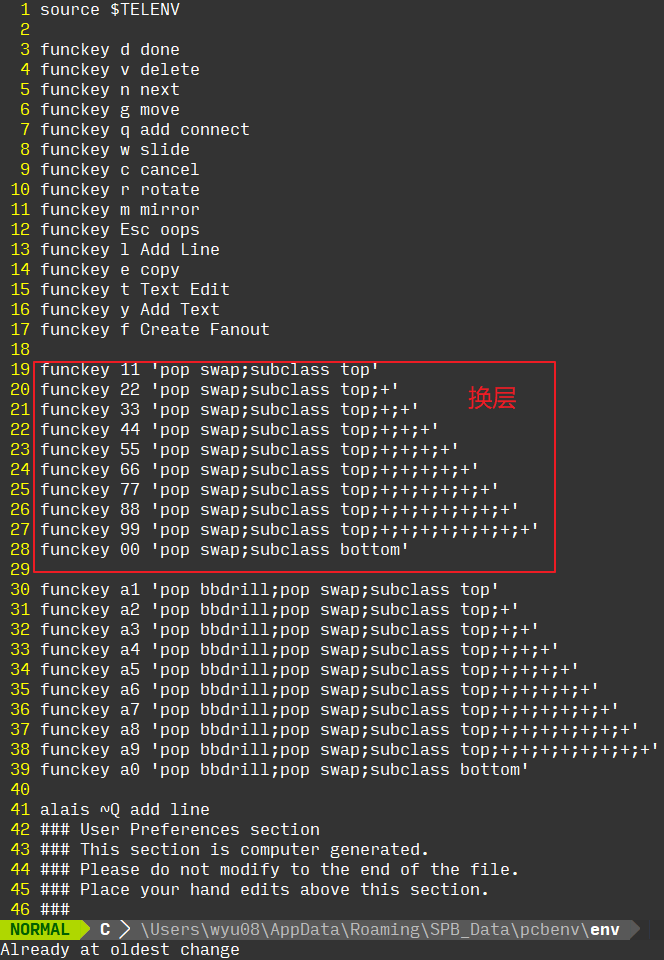
\includegraphics[width=0.4\textwidth]{figures/AllegroKey.png}

\section{钽电容画法}
此法又叫手动焊盘增大术,名字来源于\href{mailto:chl1111@mail.ustc.edu.cn}{Haolei Chen}
\subsection{电源去耦电容的作用}
通俗来说滤波电容的作用就是保证芯片供电量增大时供电能够保证,一般使用一个小的陶瓷电容配上一个大的钽电容。打个比方,两个电容就像水窖和水库,当芯片耗电量突然增加时,首先从陶瓷电容上放出电荷,WTW.
\subsection{钽电容画法}
钽电容的焊盘一般都比较大,如果还是用6mil或8mil的走线将其连到相应的电源和GND上势必会造成较大的走线电感,和钽电容的寄生电感一叠加就雪上加霜了。更重要的是,用细的走线势必要用小过孔,小过孔不仅增加电感,过大电流能力还不好,那就用大过孔+粗走线,如下图所示
\begin{figure}[htbp]
	\centering
	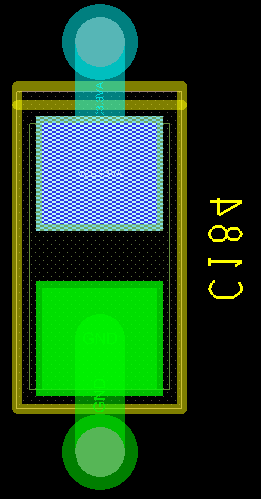
\includegraphics[width=0.3\textwidth]{figures/CapacitorWith40milVia.png}
	\label{Fig:CapacitorWith40milVia}
	\caption{用40mil走线和40mil过孔连接钽电容}
\end{figure}
\\一个钽电容用40mil的走线连到一个40mil的过孔上,问题是解决了,但是大的地孔会将地平面和电源平面打出一些洞,如果不幸有走线在这些洞附近,其地回路必然受到影响。还有更优的选项,在焊盘上铺上一层铜,然后在铜皮上打许多小过孔,这样寄生电感更小还可以塞孔,如下图所示,相当于把钽电容的焊盘增大了一部分用于打过孔。这样的方法同样适用于其他需要和内电层良好接触的表贴焊盘。
\begin{figure}[htbp]
	\centering
	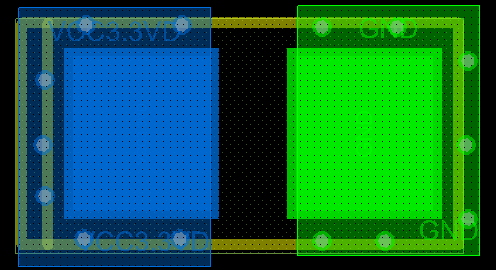
\includegraphics[width=0.3\textwidth]{figures/CapacitorWithShape.png}
	\label{fig:CapacitorWithShape}
	\caption{在钽电容焊盘上铺铜然后打小孔}
\end{figure}
\section{Allegro配色标准}
\section{盲埋孔设计}
\end{document}